%% IEEE conference submission (IEEEtran, two-column, US Letter).
%%
%% Converted from the Springer sn-jnl [iicol] build on the `main` branch of this
%% repository; that build targeted Datenbank-Spektrum and is superseded.
%% IEEEtran.cls and IEEEtran.bst are NOT vendored: they are on CTAN and tectonic
%% fetches them from the TeX Live bundle. See TEMPLATE_PROVENANCE.md.
%%
%% Single file by convention inherited from the previous build. The evidence
%% table is GENERATED INTO this file by evaluation/make_tables.py, between the
%% "% BEGIN GENERATED <name>" / "% END GENERATED <name>" markers. Do not edit
%% inside those spans by hand -- edit evaluation/capability_matrix.json and
%% re-run the generator, or the paper and the evidence will diverge.
\documentclass[conference]{IEEEtran}
\IEEEoverridecommandlockouts

\usepackage{cite}
\usepackage{amsmath,amssymb}
% IEEEtran asks for Times (ptm) shapes that are not set up under the Unicode
% encoding tectonic's engine uses, so every bold and small-caps run silently
% fell back to the default family -- \textbf produced no bold at all. newtx
% supplies the shapes properly. It must load AFTER amssymb with \Bbbk released,
% because both define that symbol and the clash is an error, not a warning.
\usepackage{newtxtext}
\let\Bbbk\relax
\usepackage{newtxmath}
\usepackage{booktabs}
\usepackage{array}
\usepackage{graphicx}
\usepackage{textcomp}
\usepackage{tikz}
\usetikzlibrary{positioning,arrows.meta,fit,backgrounds,calc}
\usepackage{stfloats}   % lets full-width floats sit at the bottom of a page
\usepackage[hidelinks]{hyperref}

\newcommand{\nd}[1]{\textsf{#1}}          % node label
\newcommand{\eg}[1]{\textsc{\small #1}}   % edge type
% Verdict marks. Only absence is bolded, so a reader scanning the capability
% tables finds the gaps rather than the successes.
\newcommand{\ry}{Y}
\newcommand{\rp}{P}
\newcommand{\rn}{\textbf{N}}
\newcommand{\rna}{--}

% Run-in headings. IEEEtran's \paragraph sets the title in the body font and
% appends a colon; these read as bold run-ins, as they did in the prior build.
\newcommand{\rih}[1]{\smallskip\noindent\textbf{#1}}

\raggedbottom

\begin{document}

\title{Operational Metadata as a Property Graph: A Reference Model and Query
Workload for Data Platform Reliability}

\author{\IEEEauthorblockN{Mogana Kumaran Sivaraman}
\IEEEauthorblockA{Senior Staff Software Engineer\\
San Francisco, CA, USA\\
Email: moganakumaran@ieee.org}
\thanks{The reference model, the synthetic lakehouse graph, all seven queries,
the validation runner and the capability matrix with its per-cell evidence are
released with this paper. The running example is synthetic: no operational
data, system names or incidents from any organisation appear in this work.}}

\maketitle

\begin{abstract}
Data platform reliability engineering asks questions that are graph
traversals: which consumers a schema change breaks, why a table is stale,
which upstream change preceded an incident, and who should be paged. The
metadata to answer them is widely captured, so the question is not whether it
exists but whether what a system \emph{represents} and what it can be
\emph{asked} suffice.

We treat this workload as a requirements instrument, specifying a
reference property graph for operational metadata --- eleven node
labels, thirteen stored relationship labels spanning fifteen typed endpoint
signatures, and one derived dataset-dependency relation, with bitemporal schema and
lineage edges --- and defining seven
reliability queries formally, each reduced to the graph operations it needs. We
validate it on an embedded property-graph engine over a synthetic lakehouse,
executing all seven against expected results fixed in advance, then
assess six metadata systems under a rubric separating representation from query
expressiveness, deriving answerability from those layers rather than judging
it directly.

All seven execute and return the expected results. None of the six
systems answered more than three of the seven, and the binding constraint
differed by system: Apache Atlas is limited by a query interface with no
traversal construct despite storing its graph in a graph database, whereas
Unity Catalog exposes the required query operations through recursive SQL,
though several workload-specific metadata elements are absent or only partially
represented. Per-hop latency, which freshness propagation needs, was
represented by none. Separating the two layers is what makes the gaps
actionable.
\end{abstract}

\begin{IEEEkeywords}
Property graphs, Data lineage, Metadata management, Data platforms,
Temporal graphs, Data reliability
\end{IEEEkeywords}

% =====================================================================
\section{Introduction}\label{sec:intro}

A pipeline fails at 02:14. The engineer paged has perhaps ten minutes before a
downstream pricing service serves stale numbers, and must answer four
questions. Which consumers are affected, and how badly? What changed upstream
shortly before the failure? Is the table stale because of this failure, or
because something three hops up has been late all night? Who owns the
component to be fixed?

Each is a question about paths through a structure: a ranked reachability
query; a temporal question, and a subtle one, since it asks what the pipeline
\emph{believed} when it ran; an aggregation along a path rather than over a
set; and a path selection with a predicate on the endpoint.

We say \emph{data platform} for the analytical stack a reliability engineer
operates --- catalog, lineage, orchestration and quality checks over a shared
store. The lakehouse is the instance the running example and the reference
implementation use; nothing in the model or the workload depends on it.

The data is largely there. A modern lakehouse~\cite{armbrust2021lakehouse,
armbrust2020delta} is surrounded by systems recording catalog entries, table
and column lineage, schema history, quality assertions, ownership and
freshness commitments. The research gap is therefore not absent metadata. It is
that answering an operational question requires two things at once --- that the
system \emph{represent} the relevant facts, and that the interface it
\emph{exposes} be able to state the required operation over them --- and that
these are routinely conflated when metadata systems are compared. A system can
hold a complete lineage graph and offer no way to aggregate along it; another
can offer a general query language over metadata that omits the quantity the
question needs.

\rih{Research questions.}
\begin{itemize}
\item[\textbf{RQ1}] What metadata structure suffices to express common
      data platform reliability investigations, and is every element of it
      required by some investigation?
\item[\textbf{RQ2}] What graph-query capabilities do they require?
\item[\textbf{RQ3}] To what extent do contemporary metadata systems expose
      those capabilities, and is the binding constraint representation or
      expressiveness?
\item[\textbf{RQ4}] Can the reference model express the workload in an
      executable graph implementation?
\end{itemize}

\rih{Contributions.} A \textbf{reference property-graph model}
(Sect.~\ref{sec:model}): eleven node labels, thirteen stored relationship
labels spanning fifteen typed endpoint signatures, and one derived
dataset-dependency relation, with schema and lineage edges carrying valid
time \emph{and} system time. A \textbf{formally
specified workload} of seven reliability queries (Sect.~\ref{sec:workload}),
each with input, output and required operations, which converts ``does this
system have lineage?'' into a question with a checkable answer. An
\textbf{executable validation} (Sect.~\ref{sec:eval}) on an embedded
property-graph engine, all seven queries checked against expectations fixed
beforehand. And a \textbf{reproducible assessment} of six systems under a
stated rubric that separates the two layers and \emph{derives} answerability
from them.

The novelty is not that metadata can be modelled as a graph --- Atlas stores
its metadata in a graph database, and DataHub and Egeria expose graph models
--- nor that column-level lineage is useful. It is the use of a reliability
workload as a \emph{requirements instrument}, and the layer separation that
instrument exposes.

\section{Background and Related Work}\label{sec:related}

\rih{Provenance.} Buneman et al.~\cite{buneman2001whywhere} separated
why- from where-provenance; Cheney et al.~\cite{cheney2009provenance} and
Herschel et al.~\cite{herschel2017survey} surveyed the field. Provenance
semirings~\cite{green2007semirings}, extended to aggregation by
Amsterdamer et al.~\cite{amsterdamer2011aggregate}, give an algebraic account
of how annotations combine along derivation paths; freshness propagation (Q4)
is an instance, with $+$ along a path and $\max$ across paths. We differ in
direction of travel: that literature is general and derives properties from
general models, whereas we fix a few operational questions and ask what
minimum structure answers them.

\rih{Metadata catalogs, and how they are compared.}
Goods~\cite{halevy2016goods} catalogued Google's datasets post hoc and found
metadata must largely be inferred rather than declared;
Ground~\cite{hellerstein2017ground} argued for a data context service spanning
application, behaviour and change. Neither offers a workload against which a
model can be judged. Comparisons of the deployed systems, meanwhile, are
typically feature inventories --- \emph{has lineage}, \emph{has column-level
lineage}, \emph{has a catalog} --- which every candidate passes, and which
therefore do not discriminate between a system that records a fact and one
that can also answer a question about it. We found no published systematic
comparison of these six against a stated reliability workload; that is an
absence we did not fill by searching, not a proof that none exists.

\rih{Graph query languages and temporal databases.} Property graphs and
their languages are well
characterised~\cite{angles2017foundations,francis2018cypher}, with GQL and
SQL/PGQ converged on a common pattern-matching core~\cite{deutsch2022gql}. The
operations our workload needs are ordinary there, so where a metadata system
cannot express them that reflects its interface, not the state of the art.
Valid and transaction time are long established, standardised as
application-time and system-time periods in SQL:2011~\cite{kulkarni2012temporal},
and temporal property graphs are active~\cite{debrouvier2021temporal} with
implementations such as GRADOOP~\cite{rost2021gradoop}. Our use is narrow and,
as far as we can determine, not standard in operational metadata: both
dimensions on lineage and schema \emph{edges}.

\rih{Schema evolution, data quality, knowledge graphs.} Schema evolution
in schema-flexible stores is well
studied~\cite{scherzinger2013nosql,klettke2015schema}, including migration cost
at scale~\cite{klettke2016migration}; the lakehouse inherits it where consumers
are pipelines. Deequ~\cite{schelter2018deequ} and TFX data
validation~\cite{breck2019validation} established declarative assertions, with
the management challenges set out by
Polyzotis et al.~\cite{polyzotis2017challenges}; we make assertions graph
citizens so \emph{coverage} becomes a reachability question. The
knowledge-graph literature~\cite{hogan2021knowledge,acosta2013crowdsourcing}
addresses heterogeneity and quality over graph data, and operational metadata
is a small, well-typed instance --- though Q7's reading of a missing assertion
is closed-world.

\rih{What this is not.} Not a lineage-visualisation or
data-observability proposal: those render a graph an operator reads, whereas
our concern is which operations must be \emph{expressible} over it --- which is
why a good lineage explorer can still leave Q4 unanswerable. Nor a new metadata
system.

\section{A Reference Model for Operational Metadata}\label{sec:model}

We model operational metadata as a directed, labelled property graph
$G = (V, E, \lambda, \pi, \tau)$ where $\lambda$ assigns labels, $\pi$ assigns
properties in the usual sense~\cite{angles2017foundations}, and $\tau$ assigns
to each temporal edge a pair of intervals defined in
Sect.~\ref{sec:bitemporal}. Table~\ref{tab:edges} gives the edges and
Fig.~\ref{fig:model} shows the whole. The justification for each element
is the query it serves; Table~\ref{tab:trace} tabulates that mapping in full,
and no element is present that serves no query.

\rih{Nodes.} Eleven labels, each carrying only the properties the
workload reads: \nd{Dataset}(\texttt{name}),
\nd{SchemaVersion}(\texttt{version\_id}, \texttt{ordinal}),
\nd{Field}(\texttt{fqn}, \texttt{data\_type}, \texttt{nullable}),
\nd{Pipeline}(\texttt{name}, \texttt{schedule\_minutes}),
\nd{Run}(\texttt{run\_id}, \texttt{scheduled\_for}, \texttt{ended\_at},
\texttt{status}, \texttt{delay\_minutes}),
\nd{QualityAssertion}(\texttt{assertion\_id}, \texttt{kind},
\texttt{severity}), \nd{AssertionResult}(\texttt{result\_id},
\texttt{outcome}, \texttt{observed\_at}), \nd{Consumer}(\texttt{name},
\texttt{criticality}), \nd{Principal}(\texttt{name}, \texttt{kind}),
\nd{SLA}(\texttt{sla\_id}, \texttt{max\_staleness\_minutes}) and
\nd{Incident}(\texttt{incident\_id}, \texttt{detected\_at}).

\begin{table}[t]
% IEEEtran sets table captions in small caps above the table, where a long one
% is unreadable; the detail sits in a note below the rules instead.
\caption{Stored relationship signatures of the reference model}
\label{tab:edges}
\scriptsize
\begin{tabular}{@{}ll>{\raggedright\arraybackslash}p{0.23\columnwidth}@{}}
\toprule
Edge & From $\rightarrow$ To & Properties \\
\midrule
\eg{reads}, \eg{writes}     & P $\rightarrow$ D   & \\
\eg{has\_schema}$\dagger$   & D $\rightarrow$ SV  & bitemporal \\
\eg{declares}               & SV $\rightarrow$ F  & \\
\eg{derives\_from}$\dagger$ & F $\rightarrow$ F   &
   \texttt{dependency}, \texttt{subtype}, bitemp. \\
\eg{instance\_of}           & R $\rightarrow$ P   & \\
\eg{produced}               & R $\rightarrow$ AR  & \\
\eg{evaluates}              & AR $\rightarrow$ QA & \\
\eg{asserts\_on}            & QA $\rightarrow$ D  & \\
\eg{asserts\_on}            & QA $\rightarrow$ F  & \\
\eg{consumes}               & C $\rightarrow$ D   & \\
\eg{owns}                   & Pr $\rightarrow$ D  & \\
\eg{owns}                   & Pr $\rightarrow$ P  & \\
\eg{governed\_by}           & D $\rightarrow$ SLA & \\
\eg{affects}                & I $\rightarrow$ D   & \\
\midrule
\eg{feeds} \emph{(deriv.)}  & D $\rightarrow$ D   &
   \texttt{via\_} \texttt{pipeline}, \texttt{latency\_} \texttt{minutes} \\
\bottomrule
\end{tabular}

\smallskip
\begin{minipage}{\columnwidth}
\scriptsize
Node labels abbreviated: \nd{D}ataset, \nd{SV} SchemaVersion, \nd{F}ield,
\nd{P}ipeline, \nd{R}un, \nd{QA} QualityAssertion, \nd{AR} AssertionResult,
\nd{C}onsumer, \nd{Pr}incipal, \nd{I}ncident. Thirteen relationship labels
span fifteen signatures: \eg{asserts\_on} and \eg{owns} each admit two
endpoint pairs and are listed once per pair. $\dagger$ marks the two
bitemporal relationships, which carry \texttt{valid\_from},
\texttt{valid\_to}, \texttt{recorded\_from} and \texttt{recorded\_to}.
\eg{feeds} is a \emph{derived} dependency relation and is not stored; its
\texttt{via\_pipeline} property identifies the \nd{Pipeline} witnessing the
dependency (Sect.~\ref{sec:derived}). Every signature here appears in
Fig.~\ref{fig:model}, and none is absent from it.
\end{minipage}
\end{table}

\rih{Design decisions.} Three labels are less usual in a catalog.
\nd{SchemaVersion} is a node rather than a property, so a schema can be
referred to, versioned and connected to the fields it declares; field
membership is consequently schema-version-dependent, reached by
\nd{Dataset}\,\eg{has\_schema}\,\nd{SchemaVersion}\,\eg{declares}\,\nd{Field},
which is what lets Q2 ask about a field a \emph{past} version declared.
\nd{Run} is separated from \nd{Pipeline}, distinguishing a definition from its
executions, without which root-cause questions cannot be posed. \nd{Consumer}
carries a \texttt{criticality} tier, so impact is ranked rather than
enumerated: an affected nightly report and an affected pricing service are not
the same event. \nd{AssertionResult} is separate from \nd{QualityAssertion},
joined by \eg{evaluates}, because Q7 asks whether an assertion \emph{exists}
and Q3 whether one \emph{failed}; collapsing them leaves one unanswerable.

\emph{Column-level lineage is a first-class edge.} \eg{derives\_from} connects
\nd{Field} to \nd{Field}, because dataset-level lineage over-approximates: it
reports that a downstream table depends on an upstream one when the question is
whether it depends on the column being dropped. We adopt OpenLineage's
\emph{direct}/\emph{indirect} distinction~\cite{olspec} in the
\texttt{dependency} property: a column used in a filter or join affects an
output without deriving it, and dropping a join key breaks a pipeline as surely
as dropping a projected column.

\subsection{Bitemporal schema and lineage}\label{sec:bitemporal}

Both bitemporal edges carry two intervals, in the sense standardised for
application and system time in SQL:2011~\cite{kulkarni2012temporal}:

\begin{IEEEdescription}[\IEEEsetlabelwidth{System time}]
\item[Valid time] $[\texttt{valid\_from},\ \texttt{valid\_to})$ --- the period
  during which the relationship held \emph{in the operational world}.
\item[System time] $[\texttt{recorded\_from},\ \texttt{recorded\_to})$ --- the
  period during which the metadata system \emph{held that belief}.
\end{IEEEdescription}

The two diverge whenever metadata arrives late or is corrected
retrospectively --- precisely the situation an incident investigation meets. In
the running example a schema change on \texttt{orders\_raw} became
operationally valid at 01:50 but was first recorded at 02:10, so a pipeline
running at 02:00 read data in the new shape while the catalog still answered
with the old schema. At the 02:14 incident two questions have two answers:

\begin{align}
\text{valid at } t &: \ \texttt{valid\_from} \le t < \texttt{valid\_to}
  \label{eq:valid}\\
\text{believed at } b &: \ \texttt{recorded\_from} \le b < \texttt{recorded\_to}
  \label{eq:tx}
\end{align}

With $t = 02{:}14$, (\ref{eq:valid}) selects the new version; with
$b = 02{:}00$, (\ref{eq:tx}) selects the old one. A single version history,
however carefully maintained, can represent one of these but not both --- and
the discrepancy is the explanation the engineer is looking for. This is why we
require both dimensions, and why Sect.~\ref{sec:eval} asks of each system
whether it represents them.

\subsection{The derived dependency relation}\label{sec:derived}

Q3, Q4, Q5 and Q7 traverse dataset-to-dataset dependency, which the model does
\emph{not} store as a primitive. Storing it would duplicate \eg{reads} and
\eg{writes} and could drift from them. We derive one edge per \emph{witness}
pipeline: for every $p$ reading $d_1$ and writing $d_2$ there is a derived
edge $e$, written $d_1 \xrightarrow{\ \text{feeds}[p]\ } d_2$, such that
\begin{equation}
\begin{split}
d_1 \xrightarrow{\ \text{feeds}[p]\ } d_2 \iff
  p \in \nd{Pipeline}\ \wedge \\
p \xrightarrow{\text{reads}} d_1 \ \wedge\
p \xrightarrow{\text{writes}} d_2
\end{split}
\label{eq:feeds}
\end{equation}

The bracketed $p$ is not a third endpoint: \eg{feeds} stays an ordinary
\nd{Dataset} $\rightarrow$ \nd{Dataset} edge and $p$ is kept as an edge
\emph{property},
\begin{equation}
\mathrm{via\_pipeline}(e) := p ,
\label{eq:via}
\end{equation}
recording which pipeline witnessed the dependency. That is what lets Q5
recover the intermediate \nd{Pipeline}: the rest of the workload needs only
dataset-to-dataset dependency, but ownership attaches to datasets \emph{and}
pipelines, so Q5 alone must reconstruct the node Eq.~(\ref{eq:feeds})
otherwise hides.

Each derived edge also carries a latency. Of the available readings ---
expected processing time, observed run delay, SLA lag, dataset freshness ---
we commit to one:

\begin{equation}
\mathrm{latency}(e) := \mathrm{delay}\big(r^{*}_{p(e)}\big)
\label{eq:latency}
\end{equation}
\begin{equation}
\mathrm{delay}(r) := r.\texttt{ended\_at} - r.\texttt{scheduled\_for}
\label{eq:delay}
\end{equation}

for a hop $e$ whose witness is $\mathrm{via\_pipeline}(e) = p$, with
$r^{*}_{p}$ the most recent \textsc{success}ful \nd{Run} of $p$. Latency and
witness therefore refer to the same pipeline by construction. Hop latency is thus the \emph{observed
delay, against schedule, of the run that materialised the downstream dataset}
--- observable, already in the model via \nd{Run}, and what an operator means
by how much lateness a hop contributes.

That it must be computed before it can be traversed is part of what makes Q4
demanding, and Sect.~\ref{sec:capability} reports that none of the systems
examined represents an equivalent quantity.

\rih{Running example.} A synthetic retail lakehouse:
\texttt{orders\_raw} and \texttt{fx\_rates} are ingested hourly;
\texttt{fx\_rates} is smoothed into \texttt{fx\_rates\_smoothed};
\texttt{clean\_orders} reads \texttt{orders\_raw} and
\texttt{fx\_rates\_smoothed} to write \texttt{orders\_clean}; and
\texttt{agg\_revenue} writes \texttt{daily\_revenue}, consumed by a pricing
service (criticality~1) and a finance dashboard (criticality~3). The example is
synthetic throughout; no operational data from any organisation appears in this
paper.

\begin{figure*}[t]
\centering
\resizebox{\textwidth}{!}{%
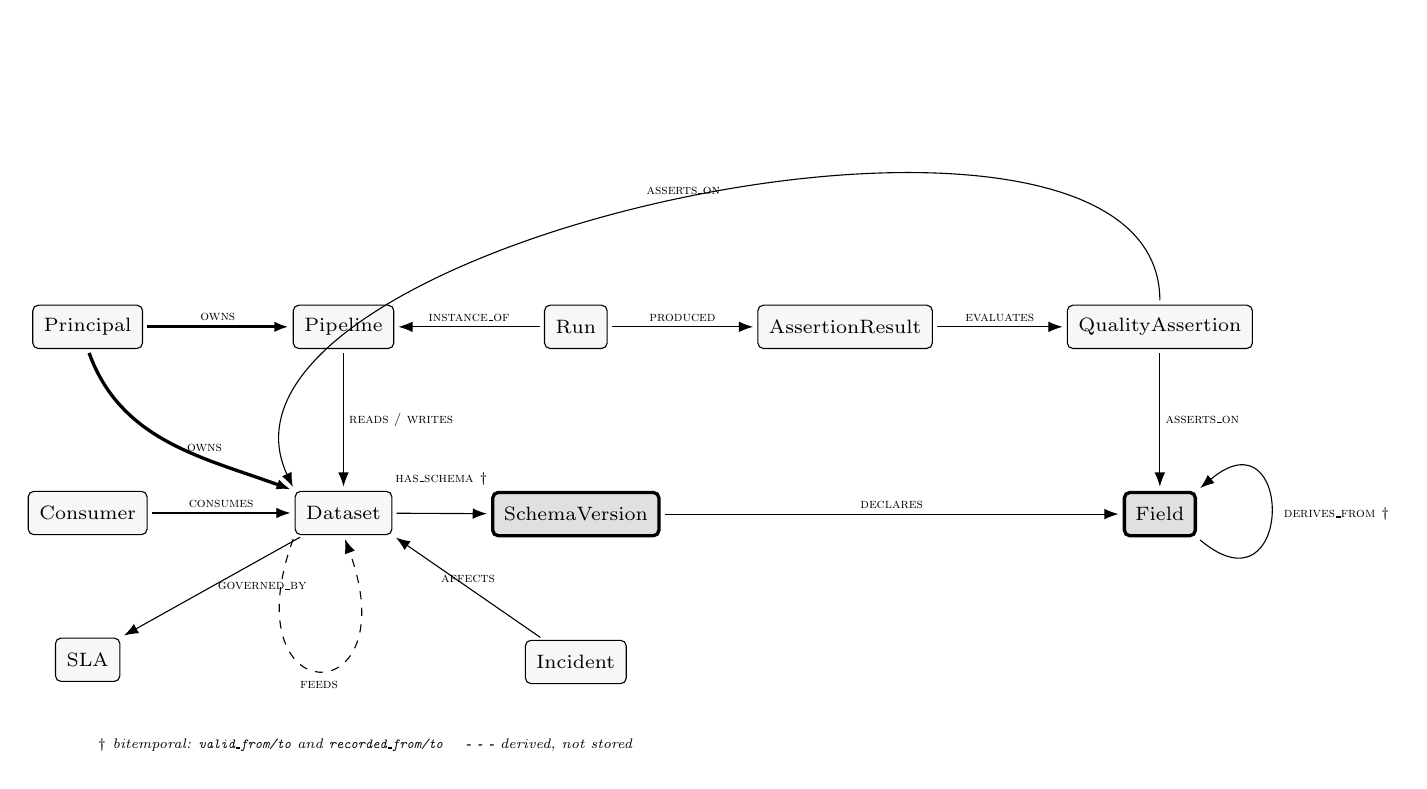
\begin{tikzpicture}[
  font=\scriptsize,
  n/.style={draw, rounded corners=2pt, minimum height=5.5mm, inner xsep=4pt,
            fill=black!3},
  t/.style={n, fill=black!12, very thick},
  e/.style={-{Latex[length=1.8mm]}, shorten >=1.5pt, shorten <=1.5pt},
  de/.style={e, dashed},
  o/.style={e, very thick},   % ownership: decides Q5
  lh/.style={font=\tiny\scshape, above=0.3mm, inner sep=1pt},
  lv/.style={font=\tiny\scshape, right=0.3mm, inner sep=1pt}
]
% row 1: execution and assertion side
\node[n]                       (prin) {Principal};
\node[n, right=19mm of prin]   (pipe) {Pipeline};
\node[n, right=19mm of pipe]   (run)  {Run};
\node[n, right=19mm of run]    (ar)   {AssertionResult};
\node[n, right=17mm of ar]     (qa)   {QualityAssertion};

% row 2: data side. Field sits under QualityAssertion so asserts_on is short.
\node[n, below=18mm of prin]   (cons) {Consumer};
\node[n, below=18mm of pipe]   (ds)   {Dataset};
\node[t, below=18mm of run]    (sv)   {SchemaVersion};
\node[t, below=18mm of qa]     (fl)   {Field};

% row 3
\node[n, below=13mm of cons]   (sla)  {SLA};
\node[n, below=13mm of sv]     (inc)  {Incident};

\draw[o] (prin) -- node[lh]{owns}         (pipe);
\draw[e] (run)  -- node[lh]{instance\_of} (pipe);
\draw[e] (run)  -- node[lh]{produced}     (ar);
\draw[e] (ar)   -- node[lh]{evaluates}    (qa);

\draw[e] (pipe) -- node[lv]{reads / writes} (ds);
\draw[e] (qa)   -- node[lv]{asserts\_on}    (fl);
% The second asserts_on endpoint. Routed over the top: taken straight it
% passed through AssertionResult and its label collided with `produced'.
\draw[e] (qa.north) to[out=90,in=115,looseness=0.8]
         node[lh,pos=0.5]{asserts\_on} (ds.north west);

\draw[e] (ds) -- node[lh, above=3.2mm, pos=0.5]{has\_schema $\dagger$} (sv);
\draw[e] (sv) -- node[lh]{declares}      (fl);
\draw[e] (cons) -- node[lh]{consumes}    (ds);
% Both `owns` signatures, drawn thicker because Q5's answer depends on which
% of them is nearer the incident. The earlier version of this figure drew
% owns: Principal -> Consumer, which the model does not contain.
\draw[o] (prin.south) to[out=-70,in=160] node[lv,pos=0.55]{owns} (ds.north west);

\draw[e] (fl.south east) to[out=-40,in=40,looseness=7]
         node[font=\tiny\scshape, right=0.5mm]{derives\_from $\dagger$}
         (fl.north east);

\draw[e] (ds)  -- node[lv]{governed\_by} (sla.north east);
\draw[e] (inc) -- node[lh, above=0.2mm]{affects} (ds.south east);

% the derived relation, dashed. Placed below-left of Dataset, where nothing
% else runs: on the west side it overlapped the `consumes' label.
\draw[de] (ds.south west) to[out=250,in=290,looseness=10]
          node[font=\tiny\scshape, below=0.3mm]{feeds} (ds.south);

\node[font=\tiny\itshape, below=6mm of sla.south, anchor=north west]
     {$\dagger$ bitemporal: \texttt{valid\_from/to} and
      \texttt{recorded\_from/to} \quad
      \textbf{- - -} derived, not stored};
\end{tikzpicture}}
\caption{The reference model. Shaded nodes are first-class here and usually
attributes in a catalog. Solid edges are stored; the \textbf{dashed} self-loop
on \nd{Dataset} is the \emph{derived} \eg{feeds} relation of
Eq.~(\ref{eq:feeds}). The two edges marked $\dagger$ are bitemporal, carrying
valid time and system time rather than a single write timestamp. Ownership is
drawn heavier because Q5's answer depends on which owned node is nearer the
incident, and \eg{owns} attaches to both datasets and pipelines. All fifteen
stored endpoint signatures of Table~\ref{tab:edges} appear here, and no
others.}
\label{fig:model}
\end{figure*}

% =====================================================================
\section{The Reliability Query Workload}\label{sec:workload}

The workload is this paper's instrument, so it is specified rather than
described. Each query below is given its input, its output and the graph
operations it requires. Table~\ref{tab:trace} maps each requirement onto the
model elements that satisfy it, which is the traceability supporting the
minimality claim: an element serving no query is not in the model.

% BEGIN GENERATED tab_trace
\begin{table*}[t]
\caption{Requirement-to-model traceability}
\label{tab:trace}
\scriptsize
\centering
\begin{tabular}{@{}l>{\raggedright\arraybackslash}p{0.20\textwidth}>{\raggedright\arraybackslash}p{0.22\textwidth}>{\raggedright\arraybackslash}p{0.34\textwidth}@{}}
\toprule
Query & Representation required & Query operation required & Reference-model elements \\
\midrule
Q1 \emph{Downstream impact} & dataset lineage, ownership & transitive closure & reads, writes, consumes; Consumer.criticality \\
Q2 \emph{Breaking change} & field-level lineage, schema versions & transitive closure, reverse traversal & derives\_from, has\_schema, declares \\
Q3 \emph{Root-cause candidates} & dataset lineage, run history, quality assertions & reverse traversal, temporal predicates & feeds (derived), instance\_of, produced, evaluates \\
Q4 \emph{Freshness propagation} & dataset lineage, per-hop latency & transitive closure, path-local aggregation & feeds (derived).latency\_minutes, governed\_by \\
Q5 \emph{Escalation routing} & dataset lineage, ownership & transitive closure, path selection & feeds (derived), owns, consumes; Consumer.criticality \\
Q6 \emph{Change attribution} & schema versions, valid time, transaction time & temporal predicates & has\_schema with valid\_from/to and recorded\_from/to; affects \\
Q7 \emph{Coverage gaps} & dataset lineage, quality assertions & transitive closure, negation under closure & feeds (derived), asserts\_on, consumes \\
\bottomrule
\end{tabular}

\smallskip
\begin{minipage}{\textwidth}
\scriptsize
Every node, edge and property of the reference model appears in the last column of some row: an element that serves no query is not in the model. Generated from \texttt{evaluation/capability\_matrix.json}.
\end{minipage}
\end{table*}
% END GENERATED tab_trace

\subsection{Workload semantics}\label{sec:semantics}

\rih{Q1 Downstream impact.}
\emph{In:} dataset $d_0$. \emph{Out:} $(c, c.\texttt{criticality})$ for every
\nd{Consumer} $c$ with $c \xrightarrow{\text{consumes}} d$ and
$d_0 \xrightarrow{\text{feeds}^{*}} d$, ordered by criticality ascending.
\emph{Requires:} transitive closure over typed edges. Q1 is the control, keeping the assessment honest about what is genuinely hard.

\rih{Q2 Breaking change.}
\emph{In:} field $f$ to be removed or retyped. \emph{Out:} every field $f'$
with $f' \xrightarrow{\text{derives\_from}^{+}} f$, with hop distance.
\emph{Requires:} field-level lineage closure plus schema versioning to resolve
$f$ against the version that declared it. The discriminating case is
\textsc{indirect} dependency: a downstream field joining on \texttt{currency}
without projecting it depends on it really, and a projection-only or
dataset-level analysis calls the change safe.

\rih{Q3 Root-cause candidates.}
\emph{In:} incident $i$, window $\Delta$. \emph{Out:} upstream datasets $u$
with $u \xrightarrow{\text{feeds}^{*}} d_0$, where
$i \xrightarrow{\text{affects}} d_0$, such that some \nd{Run} of a pipeline
writing $u$ either has $\texttt{status} = \textsc{failed}$ or \eg{produced} an
\nd{AssertionResult} with $\texttt{outcome} = \textsc{fail}$, and has
$\texttt{ended\_at} \in [i.\texttt{detected\_at} - \Delta,\
i.\texttt{detected\_at}]$. \emph{Requires:} reverse traversal and a temporal predicate on run state. The
second disjunct is why \nd{AssertionResult} and \eg{evaluates} exist: a run can
succeed and still be the cause, and traversing \eg{evaluates} to the
\nd{QualityAssertion} turns ``some assertion failed'' into a named one, which
is the difference between a signal and an action.

\rih{Q4 Freshness propagation.}
\emph{In:} dataset $d$. \emph{Out:} implied staleness, and whether it breaches
the governing \nd{SLA}. Let $\mathcal{P}(d)$ be the set of \eg{feeds} paths
ending at $d$. Then
\begin{equation}
\begin{split}
L(P) &= \sum_{e \in \mathrm{hops}(P)} \mathrm{latency}(e) \\
\mathrm{ImpliedStaleness}(d) &= \max_{P \in \mathcal{P}(d)} L(P)
\end{split}
\label{eq:q4}
\end{equation}
with $\mathrm{latency}$ as committed in Eq.~(\ref{eq:latency}).
\emph{Requires:} three capabilities usually collapsed into ``path
aggregation'' --- variable-length traversal to enumerate $\mathcal{P}(d)$, a
\emph{path-local} fold scoped to one path to compute $L(P)$, and an aggregation
\emph{across} paths for the maximum. Reachability supplies neither of the last
two: that $d$ is reachable from a delayed source says nothing about how much
delay arrives. The executed form is \texttt{evaluation/q4.cypher}; Kuzu has no
\texttt{reduce}, so the path-local fold is written
\texttt{list\_sum(list\_transform(rels(p),...))}.


\rih{Q5 Escalation routing.}
\emph{In:} incident $i$ with $i \xrightarrow{\text{affects}} d_0$. \emph{Out:}
one \nd{Principal} to page, and the node it owns. Ownership attaches to
\emph{both} datasets and pipelines, so Q5 is defined over the alternating
dependency path
\begin{equation}
d_0 \xleftarrow{\text{reads}} p_1 \xrightarrow{\text{writes}} d_1
      \xleftarrow{\text{reads}} p_2 \xrightarrow{\text{writes}} \cdots
\label{eq:altpath}
\end{equation}
rather than over \eg{feeds} alone, which collapses $p_k$ out of the path and
would make a pipeline owner unreachable. Position interleaves the two kinds:
$d_k$ sits at $2k$ and $p_{k+1}$ at $2k+1$. Then: (i)~criticality is a total
order on integers, lower more critical; (ii)~the target $c^{*}$ is the
reachable consumer of minimum criticality, ties broken by name; (iii)~among
nodes of a shortest dependency path from $d_0$ to $c^{*}$'s dataset, take the
one at minimum position carrying an \eg{owns} edge; (iv)~if several principals
own it, the lexicographically first. \emph{Requires:} path selection, and
ownership resolvable in-graph over two node kinds.

This is the one query that needs the intermediate \nd{Pipeline}, and it is why
the \eg{owns}\,:\,\nd{Principal} $\rightarrow$ \nd{Pipeline} signature is in
the model at all. Q1, Q3, Q4 and Q7 are content with \eg{feeds}; Q5 recovers
the alternating path by expanding each \eg{feeds} hop back through its witness
$\mathrm{via\_pipeline}$, Eq.~(\ref{eq:via}), since no engine in common use
offers variable-length traversal over a composite pattern.

\rih{Q6 Change attribution.}
\emph{In:} a dataset $d$, incident time $t$, belief time $b$. \emph{Out:} for
each \nd{SchemaVersion} of $d$, whether it satisfied (\ref{eq:valid}) at $t$
and whether it satisfied (\ref{eq:tx}) at $b$. In the worked example $d$ is an
\emph{upstream} dataset surfaced by Q3 rather than the incident dataset
itself, which is the usual shape of an investigation: Q3 narrows the
candidates, Q6 attributes the change on one of them.
\emph{Requires:} two independent temporal dimensions on one edge; where they
disagree, the disagreement is the finding.

\rih{Q7 Coverage gaps.}
\emph{In:} criticality threshold $k$ \emph{and an evaluation time} $t$.
\emph{Out:} pairs $(c, u)$ where $c.\texttt{criticality} \le k$,
$c \xrightarrow{\text{consumes}} d$, $u \xrightarrow{\text{feeds}^{*}} d$, and
$u$ is \emph{unasserted at} $t$. The time is not optional: because
\eg{has\_schema} is bitemporal, which fields a dataset declares is itself a
function of when one asks, so coverage is judged against the version
satisfying Eq.~(\ref{eq:valid}) at $t$. Four readings of ``unasserted'' are
available --- no assertion of any kind, none currently valid, none
\emph{passing}, or none covering the relevant field. We commit to the first,
refined to the schema in force: $u$ is unasserted at $t$ iff no
\nd{QualityAssertion} \eg{asserts\_on} $u$ \emph{and} none \eg{asserts\_on} any
\nd{Field} declared by the schema version of $u$ valid at $t$. Existence, not
outcome: a \emph{failing} assertion still counts as coverage, because Q7 asks
what is unwatched and Q3 asks what is broken. \emph{Requires:} negation
\emph{under} a transitive closure, with a temporal predicate selecting the
schema version.


% =====================================================================
\section{Assessment Method}\label{sec:method}

Applying the workload to real systems requires stated criteria, or the
resulting table is not reproducible. This section gives them.

\subsection{Two layers}\label{sec:layers}

We assess on two independent axes, because conflating them hides the
diagnosis. \emph{Metadata representation} asks whether the system records the
fact a query needs; \emph{query expressiveness} asks whether the interface it
exposes can state the required operation over what it records. A query is
answerable only if both hold, so

\begin{equation}
\begin{split}
\mathrm{answerable}(Q, S) = \min\Big(
  &\min_{r \in \mathrm{rep}(Q)} S_r, \\
  &\min_{x \in \mathrm{expr}(Q)} S_x \Big)
\end{split}
\label{eq:answer}
\end{equation}

over the order $\rn < \rp < \ry$, with $\mathrm{rep}$ and $\mathrm{expr}$ the
per-query requirements recorded in \texttt{capability\_matrix.json}.
Group~(c) of Table~\ref{tab:capability} is computed by (\ref{eq:answer})
rather than judged directly, so a reader who disputes a cell can locate the
specific representation or expressiveness finding responsible for it.

\subsection{Rubric}\label{sec:rubric}

\begin{IEEEdescription}[\IEEEsetlabelwidth{\rna\ Not applicable.}]
\item[\ry\ Native.] The capability is available through a documented interface
  of the system as shipped, without reconstructing the graph outside it.
\item[\rp\ Partial.] Available only under a material qualification, which the
  cell's reason states: connector-specific rather than a property of the core
  model, bounded, requiring a join to a separately-governed store, or
  semantically narrower than the workload needs.
\item[\rn\ Absent.] Not available through any documented or source-inspected
  interface we examined.
\item[\rna\ Not applicable.] The artefact defines no layer of this kind.
  OpenLineage specifies data and not a query surface, so grading it on
  expressiveness would be a category error.
\end{IEEEdescription}

\subsection{Systems, versions and evidence}\label{sec:systems}

Six systems: the OpenLineage specification, Apache Atlas, DataHub,
OpenMetadata, Egeria and Databricks Unity Catalog --- five open source, one
proprietary but openly documented. All assessments were made on
21~September~2026 against the most current documentation we could locate, and
against source where documentation was silent on a point the workload depends
on. Atlas was assessed against its \texttt{master} branch grammar rather than
the 2.0.0 documentation still prominent in search results, because the DSL was
rewritten after that release. The sources examined were each project's
published metadata model, query documentation and, where needed,
source~\cite{olspec,atlasdocs,datahubdocs,omdocs,egeriadocs,dbxdocs}; one
finding is version-dependent, since recursive CTEs require Databricks
Runtime~17.0 or later~\cite{dbxdocs}. Table~\ref{tab:systems} gives the
per-system versions and the evidence behind each column.

% BEGIN GENERATED tab_systems
\begin{table*}[t]
\caption{Systems assessed, versions, and evidence}
\label{tab:systems}
\scriptsize
\centering
\begin{tabular}{@{}ll>{\raggedright\arraybackslash}p{0.42\textwidth}l@{}}
\toprule
System & Kind & Version / documentation examined & Evidence \\
\midrule
OpenLineage & specification & spec, docs as of 2026-09-21 & \cite{olspec} \\
Apache Atlas & open source & master branch (post-2.5.0; 2.6.0-rc tagged) & \cite{atlasdocs} \\
DataHub & open source & docs.datahub.com, 2026-09-21 & \cite{datahubdocs} \\
OpenMetadata & open source & 1.12.x docs & \cite{omdocs} \\
Egeria & open source & egeria-project.org + odpi/egeria master & \cite{egeriadocs} \\
Unity Catalog & proprietary, openly documented & Databricks docs 2026-09-21; recursive CTE requires DBR 17.0+ & \cite{dbxdocs} \\
\bottomrule
\end{tabular}

\smallskip
\begin{minipage}{\textwidth}
\scriptsize
All assessments were made on 21 September 2026 against the most current documentation we could locate, and against source where documentation was silent on a point the workload depends on. Per-cell verdicts and reasons are in \texttt{evaluation/capability\_matrix.json}.
\end{minipage}
\end{table*}
% END GENERATED tab_systems

Every cell of Table~\ref{tab:capability} carries, in
\texttt{evaluation/capability\_matrix.json}, a verdict, a one-line reason and a
citation key; the generator refuses to emit a cell lacking a source. The tables
here are produced from that file, so no capability claim in this paper is
hand-transcribed.


Two determinations rest on source rather than prose documentation, which we
flag because it is unusual. Egeria's \texttt{InstanceProperties} declares
\texttt{effectiveFromTime} and \texttt{effectiveToTime} and
\texttt{Relationship} carries \texttt{InstanceProperties}, so its edges are
validity-dated~\cite{egeriadocs} --- which the documentation does not state. Conversely, Atlas's \texttt{AtlasClassification} declares
\texttt{validityPeriods} while \texttt{AtlasRelationship} declares only
\texttt{createTime}, \texttt{updateTime} and \texttt{version}: valid time
exists in Atlas, but on tags rather than on the edges a lineage query
walks~\cite{atlasdocs}.

% =====================================================================
\section{Evaluation}\label{sec:eval}

\subsection{Reference implementation}\label{sec:impl}

We implemented the model on \textsc{Kuzu}~0.11.3, an embedded property-graph
engine with a Cypher dialect, chosen because it runs in-process and makes the
artefact reproducible from one package install. Kuzu requires typed node and
relationship tables, so the schema file is a machine-checked statement of the
model: a query naming an undeclared edge fails at parse time rather than
silently returning nothing. That is not incidental --- an undefined
\eg{feeds} edge survived an earlier draft because nothing checked it.

The graph holds \textbf{45 nodes across 11 labels and 64 edges across 14
types}, 4 of them derived \eg{feeds} edges materialised by
Eq.~(\ref{eq:feeds}). It is deliberately small, so every expected result is
derivable by hand. It models the incident of Sect.~\ref{sec:bitemporal} --- a
failed ingest at 01:45, a schema change valid at 01:50 and recorded at 02:10, a
failing assertion at 02:02, an incident at 02:14 --- with one unasserted
upstream dataset and four distinct \eg{feeds} paths into
\texttt{daily\_revenue}.

Porting notes: Kuzu has no \texttt{reduce}, so the path-local fold is
\texttt{list\_sum(list\_transform(...))}, and an \texttt{UNWIND}ed node cannot
be rebound as a pattern, so Q5 resolves ownership by key. Neither changes the
operations required.

\subsection{Query validation (RQ4)}\label{sec:validation}

Each query was executed and compared with an expected result written down
\emph{before} the run. \textbf{All seven executed and all seven matched};
Table~\ref{tab:validation} gives the per-query capability, outcome and row
count, and the reading of each result is in
\texttt{evaluation/results.json}. This answers RQ4 affirmatively and, with the
traceability mapping, RQ2 and the sufficiency half of RQ1: the model expresses
the workload, and the operations it needs are the six in group~(b) of
Table~\ref{tab:capability}. On the other half, necessity is \emph{exhibited}
rather than proved --- every element is justified by a query that uses it, but
we do not show no smaller model exists (Sect.~\ref{sec:threats}).

% BEGIN GENERATED tab_validation
\begin{table*}[t]
\caption{Query validation on the reference implementation}
\label{tab:validation}
\scriptsize
\centering
\begin{tabular}{@{}l>{\raggedright\arraybackslash}p{0.46\textwidth}ccc@{}}
\toprule
Query & Capability exercised & Executes & Matches & Rows \\
\midrule
Q1 & transitive closure over typed edges & yes & yes & 2 \\
Q2 & column-level lineage closure with schema versioning & yes & yes & 2 \\
Q3 & reverse traversal with a temporal predicate & yes & yes & 2 \\
Q4 & variable-length traversal + path-local aggregation + aggregation across paths & yes & yes & 1 \\
Q5 & path selection over the alternating dataset-pipeline path, with in-graph ownership & yes & yes & 1 \\
Q6 & two independent temporal dimensions on one edge & yes & yes & 2 \\
Q7 & negation applied under a transitive closure & yes & yes & 1 \\
\bottomrule
\end{tabular}

\smallskip
\begin{minipage}{\textwidth}
\scriptsize
Each query executed against the synthetic graph on Kuzu 0.11.3. \emph{Matches} means the returned rows equalled an expectation fixed in \texttt{evaluation/run\_validation.py} \emph{before} the run. Per-query readings are in \texttt{evaluation/results.json}.
\end{minipage}
\end{table*}
% END GENERATED tab_validation


Three results are worth reading rather than counting. Q4 instantiates Eq.~(\ref{eq:q4}) and
returns an implied staleness of \textbf{36 minutes against a 30-minute SLA},
from \texttt{fx\_rates} $\to$ \texttt{fx\_rates\_smoothed} $\to$
\texttt{orders\_clean} $\to$ \texttt{daily\_revenue} accumulating $20+12+4$.
The other three paths into \texttt{daily\_revenue} total 16, 16 and 4, so
neither reachability nor a per-dataset freshness value surfaces the breach ---
only the path-local sum followed by the cross-path maximum does. The 4-minute
single-hop path makes the point sharply: a dataset one hop from the target can
look timely while the graph behind it is half an hour late. Q6 returns both schema versions with
opposite verdicts --- v2 valid at the incident but not believed at 02:00, v1
believed then but no longer valid. Q7, evaluated at 02:14, returns one pair: the tier-1 pricing service and
\texttt{fx\_rates}, three hops upstream and unasserted under the schema valid
at that instant. Q5 returns a \emph{pipeline} owner: the incident dataset
\texttt{orders\_clean} is unowned, so the nearest owned node on the dependency
path is \texttt{agg\_revenue} at position~1, owned by the on-call rotation ---
nearer than \texttt{daily\_revenue}'s own owner at position~2. Traversing only
\eg{feeds} would have collapsed that pipeline out of the path and paged the
wrong team.

What this does \emph{not} show: no timings were taken and none should be
inferred. The graph is orders of magnitude smaller than a real catalog, and a
capability expressible here may be impractical at scale.

\subsection{Capability assessment (RQ3)}\label{sec:capability}

Table~\ref{tab:capability} gives both assessed layers and, in its third
group, the answerability derived from them by Eq.~(\ref{eq:answer}).

% BEGIN GENERATED tab_capability
\begin{table*}[t]
\caption{Capability assessment of six metadata systems}
\label{tab:capability}
\scriptsize
\centering
\begin{tabular}{@{}lcccccc@{}}
\toprule
 & OpenL. & Atlas & DataHub & OpenM. & Egeria & UC \\
\midrule
\multicolumn{7}{@{}l}{\textbf{(a) Metadata representation \emph{-- does the system record it?}}} \\[1pt]
\quad dataset lineage & \ry & \ry & \ry & \ry & \ry & \ry \\
\quad field-level lineage & \ry & \rp & \ry & \ry & \ry & \rp \\
\quad schema versions & \ry & \rp & \ry & \ry & \ry & \rn \\
\quad run history & \ry & \rp & \ry & \ry & \rp & \rp \\
\quad quality assertions & \ry & \rn & \ry & \ry & \rp & \rp \\
\quad ownership & \rn & \ry & \ry & \ry & \ry & \ry \\
\quad per-hop latency & \rn & \rn & \rn & \rn & \rn & \rn \\
\quad valid time & \rn & \rp & \rn & \rn & \ry & \rn \\
\quad transaction time & \rp & \ry & \ry & \ry & \ry & \rp \\
\addlinespace[3pt]
\midrule
\multicolumn{7}{@{}l}{\textbf{(b) Query expressiveness \emph{-- can its interface ask?}}} \\[1pt]
\quad transitive closure & \rna & \rn & \ry & \rp & \ry & \ry \\
\quad reverse traversal & \rna & \rn & \ry & \rp & \ry & \ry \\
\quad path-local aggregation & \rna & \rn & \rn & \rn & \rn & \ry \\
\quad path selection & \rna & \rn & \rn & \rn & \rp & \ry \\
\quad temporal predicates & \rna & \rp & \ry & \rp & \ry & \ry \\
\quad negation under closure & \rna & \rn & \rn & \rp & \rn & \ry \\
\addlinespace[3pt]
\midrule
\multicolumn{7}{@{}l}{\textbf{(c) Workload answerability \emph{-- derived from (a) and (b) by Eq.~(\ref{eq:answer})}}} \\[1pt]
\quad Q1 Downstream impact & \rna & \rn & \ry & \rp & \ry & \ry \\
\quad Q2 Breaking change & \rna & \rn & \ry & \rp & \ry & \rn \\
\quad Q3 Root-cause candidates & \rna & \rn & \ry & \rp & \rp & \rp \\
\quad Q4 Freshness propagation & \rna & \rn & \rn & \rn & \rn & \rn \\
\quad Q5 Escalation routing & \rna & \rn & \rn & \rn & \rp & \ry \\
\quad Q6 Change attribution & \rna & \rp & \rn & \rn & \ry & \rn \\
\quad Q7 Coverage gaps & \rna & \rn & \rn & \rp & \rn & \rp \\
\bottomrule
\end{tabular}

\smallskip
\begin{minipage}{\textwidth}
\scriptsize
\ry~native, \rp~partial, \rn~absent, \rna~not applicable (OpenLineage specifies data, not a query surface). A query needs its facts from (a) \emph{and} its operations from (b); group~(c) is \emph{computed} from the two above it by Eq.~(\ref{eq:answer}), not assessed directly, so a disputed verdict there traces to a specific cell above. Groups (a) and (b) are generated from \texttt{evaluation/capability\_matrix.json}, where every cell carries a reason and a source.
\end{minipage}
\end{table*}
% END GENERATED tab_capability



\rih{Field-level lineage is comparatively mature.} Four of six represent
it natively, the specification most richly: OpenLineage's
\texttt{columnLineage} facet distinguishes \texttt{DIRECT} from
\texttt{INDIRECT} with subtypes down to \texttt{JOIN}, \texttt{FILTER} and
\texttt{WINDOW}~\cite{olspec}. DataHub carries \texttt{fineGrainedLineages}
inside \texttt{upstreamLineage}~\cite{datahubdocs}, OpenMetadata's edges carry
\texttt{columnsLineage}~\cite{omdocs}, and Egeria's \texttt{DataMapping} maps a
schema attribute of one asset to another~\cite{egeriadocs}. Atlas scores \rp\
because \texttt{ColumnLineageProcess} arrives through the Hive bridge rather
than the core type system~\cite{atlasdocs}; Unity Catalog scores \rp\ for a
documented reason bearing on Q2 --- \emph{``Lineage is not preserved for
renamed catalogs, schemas, tables, views, or columns''}~\cite{dbxdocs} ---
since a rename is exactly the change the query concerns.

\rih{The binding constraint differs by system, which is the main
finding.} Atlas is limited by \emph{expressiveness}: its current DSL grammar
contains no traversal production at all --- the \texttt{loop} and
\texttt{withPath} clauses of the pre-1.0 language are absent from both lexer
and parser grammar on \texttt{master}, the surviving aggregates apply to a
result set with no path context, and Gremlin executes DSL internally but is not
exposed~\cite{atlasdocs}. Atlas stores its metadata in a graph database and
still cannot express Q1, which is why the useful distinction is the interface
rather than the storage engine.

Unity Catalog is the mirror image, limited by \emph{representation}. Databricks
SQL supports \texttt{WITH RECURSIVE} from Databricks Runtime~17.0, with a
default limit of 100 recursion levels and a one-million-row
bound~\cite{dbxdocs}, so a recursive CTE over
\texttt{system.access.table\_lineage} expresses each operation in group~(b):
closure and reverse traversal by choice of join direction, a path-local fold
because a recursive CTE carries columns forward on each iteration, path
selection because recursion depth is an ordinary column, temporal predicates
as ordinary SQL inside the recursive step, and negation because
\texttt{NOT EXISTS} can be applied to the materialised result. Among the evaluated executable interfaces, Databricks SQL is the one that
exposes all six query-operation classes the workload uses; what it lacks is
what to point them at.

Its data-quality position is narrower than it first appears, and we revised it
during this pass. The system table
\texttt{data\_quality\_}\allowbreak\texttt{monitoring.table\_results} records
freshness and completeness \emph{results} per table, which corresponds to
\nd{AssertionResult}. There is no companion table of check
\emph{definitions}: anomaly detection is inferred from a table's own history
rather than authored, enabled per schema or catalog rather than declared per
check, and table-scoped, with no column-level checks. Nothing corresponds to
\nd{QualityAssertion}, so the cell is \rp~\cite{dbxdocs} --- and that single
change moves Q3 and Q7 from \rn\ to \rp\ by Eq.~(\ref{eq:answer}). We did not
touch those verdicts; the derivation did.

Run history is \rp\ for a subtler reason. No join between
\texttt{job\_run\_timeline} and the lineage tables is documented --- the
documented joins are to \texttt{lakeflow.jobs}, \texttt{billing.usage} and
\texttt{compute.clusters} on \texttt{workspace\_id}, \texttt{job\_id} and
\texttt{run\_id} --- but a table-to-job association exists elsewhere:
\texttt{upstream\_jobs} carries \texttt{job\_id} and \texttt{workspace\_id}
beside the table identity, exactly those keys. The cell stays \rp\ because
that path needs anomaly detection enabled and covers only monitored
tables, not because no mapping exists~\cite{dbxdocs}.

\rih{Per-hop latency is represented by none of the six, and that is why
Q4 fails everywhere.} The Q4 row of Table~\ref{tab:capability}(c) is uniformly
\rn, and the derivation locates the cause as a representation gap, not a query
gap. DataHub comes closest with a \texttt{FRESHNESS} assertion
type~\cite{datahubdocs}, and Unity Catalog reports commit freshness as
predicted versus actual commit time~\cite{dbxdocs} --- but both are per-table
staleness signals, not a latency attributed to a dependency edge, so neither
accumulates along a path. For Unity Catalog the query would be expressible the
moment the quantity existed. We had supposed every ingredient for Q4 was stored
somewhere in the set; separating the layers showed otherwise, and we record the
correction rather than dropping the claim.

\rih{Temporal semantics are uneven.} Egeria alone satisfied our
bitemporal criterion, on both nodes and edges~\cite{egeriadocs}. DataHub and
OpenMetadata record system time well --- versioned aspects, and
\texttt{major.minor} entity versions incrementing the major on column
deletion~\cite{omdocs} --- but not valid time, so they answer ``when did the
metadata change'' rather than ``what was in force''. Unity Catalog's lineage
rows carry \texttt{event\_time} under a rolling one-year retention
window~\cite{dbxdocs}.

\rih{No system answered more than three of the seven.} DataHub answers
Q1--Q3, Egeria Q1, Q2 and Q6, and Unity Catalog Q1 and Q5 with Q3 and Q7
partial. Of the remainder, OpenMetadata reaches \rp\ on four of the seven ---
more partials than any other system --- and is limited on the query layer
rather than the data, while Atlas reaches \rp\ on one. OpenLineage receives no workload verdict: it defines no query layer, so
Eq.~(\ref{eq:answer}) does not apply, and reading that as \emph{answers
nothing} would confuse a specification with an implementation. DataHub and Egeria each answer three queries natively, but not the same three,
and their partial verdicts differ again. We draw no ranking: what matters to a
reader choosing a stack is how capabilities are distributed against their own
workload, not an aggregate score.

\subsection{Threats to validity}\label{sec:threats}

\rih{Construct validity.} The workload is seven queries from
practitioner experience, not sampled from a measured incident corpus; a
different seven would produce a different table. We expect the Q4 row to be
robust, since it depends on a quantity none of the systems represents, but that
is an expectation, not a result. Our formalisations also fix choices reasonable
practitioners would make differently --- one reading of latency out of four
(Eq.~\ref{eq:latency}), one of four readings of ``unasserted'', one
tie-breaking rule in Q5 --- each stated where it is made so a reader can
substitute their own.

\rih{Internal validity.} The implementation shows the model can express
the workload; it does not establish minimality, only that a query exists for
every element. Expected results were fixed before execution, but written by the
same author as the queries.

\rih{External validity.} Synthetic validation at 45 nodes says nothing
about production behaviour, and there is no performance evaluation here at all.
A capability marked \ry\ may be prohibitively expensive on a real catalog, and
one marked \rn\ may be irrelevant to workloads other than this one.

\rih{Product-version drift.} Five systems are actively developed and the
sixth is a specification under revision. Assessments are dated
21~September~2026 and cite the artefact they rest on, but some will age: the
recursive-CTE finding is itself a capability that post-dates Databricks
Runtime~17.0. Our first pass cited Atlas~2.0.0 documentation, which predates
the DSL rewrite; re-checking against \texttt{master} changed the conclusion,
and the same risk applies to cells not re-checked as recently.

\rih{Source limitations.} We assess documented and source-inspected
interfaces. A system may have undocumented internal capabilities, and a
proprietary system may expose more to its own operators than its public
documentation shows. Absence of evidence in documentation is reported as
absence of a \emph{documented} capability, which is the claim the rubric makes.

\section{Discussion}\label{sec:discussion}

Four implications follow from the evidence, and one caution.

\rih{Representation and expressiveness should be assessed separately.}
This is the methodological point, and it changed our own conclusions. On a
single axis Atlas and Unity Catalog both look like partial performers; on two
axes they are opposite failures with opposite remedies --- Atlas needs a query
surface over a graph it already stores, Unity Catalog needs metadata to point
an already-capable surface at. Advice not distinguishing these is not
actionable.

\rih{The gap is often narrower than it appears.} For Unity Catalog,
all five queries it does not answer outright are bound by representation
rather than by recursive SQL: the traversal machinery is present, and what is
missing is schema versions, valid time, per-hop latency and assertion
definitions. For the systems
limited by expressiveness, GQL and SQL/PGQ standardised exactly the operations
needed~\cite{deutsch2022gql}, and the semiring account of aggregation along
paths is nearly two decades
old~\cite{green2007semirings,amsterdamer2011aggregate}. Little here awaits
invention.

\rih{A thin query layer may be enough.} We are \emph{not} arguing that
metadata platforms should be replaced by native graph databases: Atlas already
is one internally and scores worst here, which is the cleanest evidence that
the storage engine is not the lever. A metadata system exposing its existing
graph through a standard pattern-matching language, rather than a bespoke
fixed-depth lineage endpoint, would gain Q1, Q4, Q5 and Q7 without changing how
it stores anything.

\rih{Temporal modelling is where new representation is needed.} Valid
time on lineage and schema edges cannot be retrofitted by a better interface.
Egeria shows it is implementable within an open metadata standard, and since
Egeria already consumes OpenLineage events, the components of a bitemporal
lineage graph over platform metadata exist in one ecosystem unassembled. Per-hop
latency is the other missing quantity, and cheaper: the model derives it from
run delay orchestrators already record.

\rih{A caution.} Nothing here establishes that these are the right seven
queries, only that an organisation needing these answers must have a metadata
stack that represents and can ask for them.

% =====================================================================
\section{Limitations and Conclusion}\label{sec:conclusion}

\rih{Limitations.} Consolidating Sect.~\ref{sec:threats}: the validation
is synthetic and small; there is no latency or throughput measurement; the
workload is seven queries from experience rather than a formal incident corpus;
the sample is six systems, so proprietary platforms that may have solved parts
of this privately are unrepresented; the assessment interprets documentation
and source at one date for rapidly evolving systems; and several formal choices
are defensible rather than uniquely correct.

\rih{Conclusion.} Data platform reliability questions form a graph workload
naturally, and writing them down formally exposes what a metadata layer must
support: seven queries reduce to six graph operations over eleven node labels
and fifteen stored endpoint signatures, and the reference model expresses all
seven when executed. A compact workload is a usable requirements instrument, converting an
unfalsifiable question about features into a checkable one about operations,
and it is the part of this work most readily reused with a different set of
queries. The practical gap in contemporary systems lies less between metadata
captured and metadata missing than between metadata captured and metadata that
can be \emph{operationally queried}: among the six examined, the binding
constraint was expressiveness for some and representation for others, and none
answered more than three of the seven.

\rih{Future work.} A workload derived from a real
incident corpus would let the queries be weighted by how often they are asked;
beyond that, a scalability benchmark on catalog-sized graphs, incremental
maintenance of the derived dependency relation under continuous ingestion, and
integration with observability systems that already hold the run-delay data Q4
needs. Whether agents can be trusted to run such queries and act on the results
during an incident is a further question this paper does not address. The
capability table reported here is generated from the per-cell evidence rather
than transcribed, and that evidence is released with the artefact.

\bibliographystyle{IEEEtran}
\bibliography{references}

\end{document}
